
\documentclass[conference]{IEEEtran}

% =====================================================
% PACKAGES
% =====================================================
\usepackage[T1]{fontenc}
\usepackage{cite}
\usepackage{graphicx}
\usepackage{url}
\usepackage{amsmath}
\usepackage{array}
\usepackage{booktabs}
\usepackage{tikz}
\usepackage{listings}
\usepackage{xcolor}

\usetikzlibrary{
    arrows.meta,
    positioning,
    shapes.geometric,
    fit,
    backgrounds,
    calc
}

% =====================================================
% CODE LISTING STYLE
% =====================================================
\lstdefinestyle{miniforge}{
    basicstyle=\ttfamily\footnotesize,
    breaklines=true,
    frame=single,
    numbers=left,
    numberstyle=\tiny,
    showstringspaces=false,
    tabsize=4
}

% =====================================================
% TITLE AND AUTHOR
% =====================================================
\title{MiniForge: Design and Implementation of a Custom Interpreted Programming Language Using C++}

\author{
\IEEEauthorblockN{Chethana Sri}
\IEEEauthorblockA{
Department of Computer Technology\\
Madras Institute of Technology, Anna University\\
Chennai, India
}
}

\begin{document}

\maketitle

% =====================================================
% ABSTRACT
% =====================================================
\begin{abstract}

Programming language implementation involves several
interconnected stages, including lexical analysis,
syntax parsing, semantic analysis, runtime evaluation,
and error handling. Understanding how these stages
interact is essential for studying programming language
design and interpreter construction.

This paper presents MiniForge, a custom interpreted
programming language implemented in C++17. The project
provides a complete language-processing pipeline
consisting of a lexical analyzer, recursive-descent
parser, abstract syntax tree, semantic analyzer,
and tree-walk interpreter.

The language supports variables, data types, arithmetic
and logical expressions, conditional statements,
loops, functions, recursion, arrays, lexical scopes,
closures, and built-in functions. It also provides
an interactive read-eval-print loop (REPL), source
file execution using the .mf extension, and debugging
facilities such as execution tracing.

The implementation follows a modular architecture
in which source code is transformed into tokens,
parsed into an abstract syntax tree, checked for
semantic consistency, and evaluated by the runtime
environment. The project is organized using C++17
and CMake, with automated testing using GoogleTest
and custom test cases.

Reported validation includes successful C++ compilation
and five passing tests. This paper describes the
language architecture, implementation methodology,
supported features, evaluation results, limitations,
and possible future extensions.

\end{abstract}

\begin{IEEEkeywords}
Programming Languages, Interpreter Design, Lexical
Analysis, Recursive Descent Parsing, Abstract Syntax
Tree, Semantic Analysis, Tree-Walk Interpreter,
C++17, Programming Language Implementation.
\end{IEEEkeywords}

% =====================================================
% I. INTRODUCTION
% =====================================================
\section{Introduction}

Programming languages provide abstractions that allow
developers to express computational instructions in
a structured and understandable form.

The implementation of a programming language requires
multiple processing stages that transform source
characters into executable behavior. These stages
commonly include lexical analysis, syntax analysis,
semantic processing, and execution \cite{aho,dragon,crafting}.

A programming language interpreter executes source
programs by evaluating their representations rather
than necessarily translating them into native machine
instructions.

Building an interpreter provides practical insight
into language grammar, parsing strategies, abstract
syntax trees, variable environments, function calls,
scope management, and runtime behavior.

MiniForge is a custom interpreted programming language
developed in C++17 to explore these concepts through
a modular implementation.

The project uses a handwritten lexer, a recursive-descent
parser, an abstract syntax tree representation, a
semantic analysis stage, and a tree-walk interpreter.

\subsection{Motivation}

Many programming language concepts are initially studied
as separate theoretical topics. However, understanding
their interaction requires implementing the complete
processing pipeline.

MiniForge was developed to connect these theoretical
concepts with a practical programming language
implementation.

The project focuses on building a small but extensible
language in which fundamental programming constructs
can be expressed and executed.

\subsection{Research Objectives}

The main objectives of MiniForge are:

\begin{itemize}
    \item Design a custom programming language syntax.
    \item Implement lexical analysis and tokenization.
    \item Develop a recursive-descent parser.
    \item Represent programs using an abstract syntax tree.
    \item Perform semantic analysis and validation.
    \item Implement a tree-walk execution engine.
    \item Support variables, functions, recursion, and arrays.
    \item Implement lexical scopes and closures.
    \item Provide an interactive REPL and source-file execution.
    \item Establish automated tests for language functionality.
\end{itemize}

\subsection{Scope}

MiniForge is an interpreted language implemented in C++17.

Its execution model is based on direct evaluation of
the abstract syntax tree.

The current implementation does not include a bytecode
virtual machine, native machine-code generation, or an
optimizing compiler backend. These are considered
possible future extensions.

% =====================================================
% II. RELATED WORK
% =====================================================
\section{Background and Related Work}

\subsection{Compiler and Interpreter Design}

Compiler construction involves translating source
programs through multiple intermediate representations.
The classical compiler architecture separates lexical
analysis, syntax analysis, semantic processing,
intermediate representation, and code generation
\cite{aho,dragon,cooper}.

Although MiniForge uses interpretation rather than
native code generation, it adopts several of the
same front-end concepts.

\subsection{Lexical Analysis}

Lexical analysis transforms a sequence of source
characters into tokens representing identifiers,
keywords, operators, literals, and punctuation.

The lexical analyzer provides a structured input
sequence for the parser \cite{aho,crafting}.

\subsection{Recursive-Descent Parsing}

Recursive-descent parsing is a top-down parsing
approach in which grammar constructs are implemented
using recursive procedures.

LLVM's language implementation tutorial demonstrates
the construction of a parser and abstract syntax tree
using recursive-descent techniques and operator
precedence handling \cite{llvm}.

MiniForge follows a handwritten recursive-descent
approach for its syntax processing.

\subsection{Abstract Syntax Trees}

An abstract syntax tree represents the structural
meaning of a program while removing unnecessary
syntactic details.

AST representations are widely used in interpreters
and compilers because they simplify subsequent
analysis and execution stages \cite{aho,crafting}.

\subsection{Semantic Analysis and Type Systems}

Syntactic correctness alone does not guarantee that
a program is meaningful.

Semantic analysis examines program constructs for
validity, including variable usage, type consistency,
and function-related rules.

Type systems provide formal methods for describing
and reasoning about valid program expressions
\cite{pierce,types}.

\subsection{Interpreters and Runtime Environments}

An interpreter evaluates program constructs using
runtime representations of values and environments.

The environment associates identifiers with their
corresponding values and supports variable lookup
during execution \cite{sicp,crafting}.

\subsection{Closures and Lexical Scope}

Lexical scoping determines variable visibility based
on the structure of the source program.

Closures preserve access to variables from their
surrounding lexical environment, even when functions
are evaluated outside their original declaration
context \cite{sicp,appel,crafting}.

\subsection{C++ Implementation}

C++ provides object-oriented and generic programming
features suitable for constructing modular language
implementations.

The C++ language standard defines the facilities used
for implementing the project's token representations,
AST structures, runtime objects, and interpreter
components \cite{cppstandard,stroustrup}.

% =====================================================
% III. PROBLEM STATEMENT
% =====================================================
\section{Problem Statement}

Understanding the internal operation of programming
languages requires more than writing programs using
existing compilers and interpreters.

A practical implementation must address several
interdependent problems:

\begin{itemize}
    \item Converting source characters into meaningful tokens.
    \item Recognizing valid grammatical structures.
    \item Representing expressions and statements.
    \item Detecting semantic inconsistencies.
    \item Maintaining variable environments and scopes.
    \item Evaluating expressions and controlling execution.
    \item Handling runtime errors and invalid operations.
\end{itemize}

MiniForge addresses these challenges through a modular
interpreted language implementation.

The objective is to provide an extensible language
architecture in which each processing stage has a
clearly defined responsibility.

% =====================================================
% IV. SYSTEM ARCHITECTURE
% =====================================================
\section{System Architecture}

MiniForge follows a sequential language-processing
architecture.

Source code enters through the REPL or file execution
interface. The lexer converts characters into tokens,
the parser constructs an AST, semantic analysis
examines the resulting structures, and the interpreter
evaluates the program using runtime environments.

The architecture separates syntax processing,
semantic validation, and execution.

\subsection{Architectural Diagram}

Fig.~\ref{fig:architecture} illustrates the overall
architecture of MiniForge.

\begin{figure*}[!t]
\centering

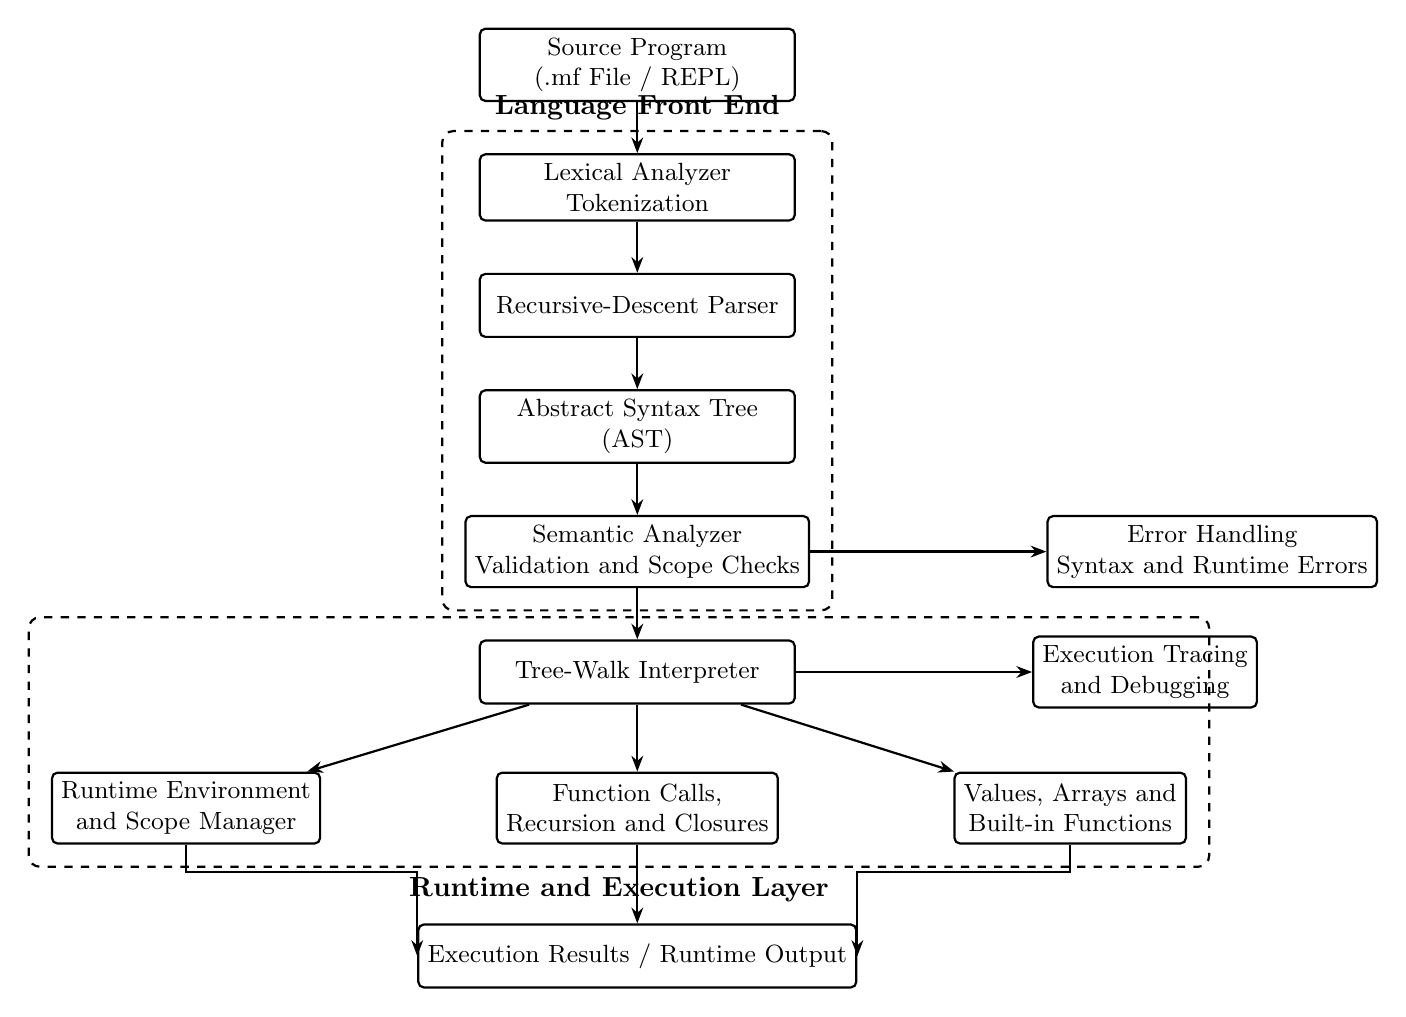
\begin{tikzpicture}[
    font=\small,
    block/.style={
        draw=black,
        rounded corners=2pt,
        thick,
        minimum width=3.2cm,
        minimum height=0.8cm,
        align=center
    },
    module/.style={
        draw=black,
        rounded corners=2pt,
        thick,
        minimum width=2.65cm,
        minimum height=0.9cm,
        align=center
    },
    arrow/.style={
        -{Stealth[length=2mm]},
        thick
    },
    boundary/.style={
        draw=black,
        dashed,
        rounded corners=4pt,
        thick,
        inner sep=8pt
    }
]

% Input
\node[block, minimum width=4.0cm] (source)
{Source Program\\(.mf File / REPL)};

% Lexer
\node[block, below=0.65cm of source,
minimum width=4.0cm] (lexer)
{Lexical Analyzer\\Tokenization};

% Parser
\node[block, below=0.65cm of lexer,
minimum width=4.0cm] (parser)
{Recursive-Descent Parser};

% AST
\node[block, below=0.65cm of parser,
minimum width=4.0cm] (ast)
{Abstract Syntax Tree\\(AST)};

% Semantic analyzer
\node[block, below=0.65cm of ast,
minimum width=4.0cm] (semantic)
{Semantic Analyzer\\Validation and Scope Checks};

% Interpreter
\node[block, below=0.65cm of semantic,
minimum width=4.0cm] (interpreter)
{Tree-Walk Interpreter};

% Runtime modules
\node[module, below left=0.85cm and 2.0cm of interpreter]
(environment)
{Runtime Environment\\and Scope Manager};

\node[module, below=0.85cm of interpreter]
(functions)
{Function Calls,\\Recursion and Closures};

\node[module, below right=0.85cm and 2.0cm of interpreter]
(values)
{Values, Arrays and\\Built-in Functions};

% Output
\node[block, below=1.0cm of functions,
minimum width=4.0cm] (output)
{Execution Results / Runtime Output};

% Error handling
\node[module, right=3.0cm of semantic]
(errors)
{Error Handling\\Syntax and Runtime Errors};

% Tracing
\node[module, right=3.0cm of interpreter]
(tracing)
{Execution Tracing\\and Debugging};

% Main flow
\draw[arrow] (source) -- (lexer);
\draw[arrow] (lexer) -- (parser);
\draw[arrow] (parser) -- (ast);
\draw[arrow] (ast) -- (semantic);
\draw[arrow] (semantic) -- (interpreter);

% Runtime connections
\draw[arrow] (interpreter) -- (environment);
\draw[arrow] (interpreter) -- (functions);
\draw[arrow] (interpreter) -- (values);

% Runtime to output
\draw[arrow] (environment.south) -- ++(0,-0.35) -| (output.west);
\draw[arrow] (functions.south) -- (output.north);
\draw[arrow] (values.south) -- ++(0,-0.35) -| (output.east);

% Error and tracing
\draw[arrow] (semantic.east) -- (errors.west);
\draw[arrow] (interpreter.east) -- (tracing.west);

% Processing boundary
\begin{scope}[on background layer]
\node[boundary,
fit=(lexer)(parser)(ast)(semantic),
label={[font=\bfseries]above:Language Front End}
] {};

\node[boundary,
fit=(interpreter)(environment)(functions)(values),
label={[font=\bfseries]below:Runtime and Execution Layer}
] {};
\end{scope}

\end{tikzpicture}

\caption{Modular architecture of the MiniForge interpreted
programming language.}
\label{fig:architecture}

\end{figure*}

\subsection{Source Input Interface}

MiniForge accepts programs through two primary
execution modes:

\begin{itemize}
    \item Interactive execution through the REPL.
    \item Source-file execution using the .mf extension.
\end{itemize}

Both modes supply source text to the language
processing pipeline.

\subsection{Lexical Analyzer}

The lexer reads source characters and groups them
into tokens.

Tokens represent language elements such as:

\begin{itemize}
    \item Identifiers and keywords.
    \item Numeric and other supported literals.
    \item Arithmetic and logical operators.
    \item Assignment operators.
    \item Delimiters and punctuation.
\end{itemize}

The token sequence is passed to the parser.

\subsection{Recursive-Descent Parser}

The parser consumes tokens according to the language
grammar.

It constructs an AST representing expressions,
declarations, statements, and other supported
language constructs.

The recursive-descent approach provides a direct
relationship between grammar rules and parser
procedures.

\subsection{Abstract Syntax Tree}

The AST represents the hierarchical structure of
the source program.

Expressions and statements are represented as
appropriate nodes, allowing later stages to examine
and evaluate program constructs without processing
the original source text again.

\subsection{Semantic Analyzer}

The semantic analyzer examines parsed constructs
for semantic validity.

Its responsibilities include the semantic checks
supported by the implementation, such as variable
and type-related validation.

\subsection{Tree-Walk Interpreter}

The interpreter evaluates AST nodes directly.

It processes expressions, executes statements,
maintains runtime environments, and handles
function invocation.

The tree-walk execution model avoids the need
for a separate bytecode generation stage.

\subsection{Runtime Environment}

The runtime environment stores variable bindings
and supports lexical scope management.

Nested environments allow identifiers to be
resolved according to their visibility within
the program.

\subsection{Function and Closure Support}

MiniForge supports function declarations, function
calls, recursion, and closures.

Closures preserve access to the appropriate
surrounding lexical environment.

\subsection{Error Handling and Tracing}

The implementation includes error handling for
invalid language constructs and runtime failures.

Execution tracing provides additional visibility
into interpreter behavior during debugging.

% =====================================================
% V. LANGUAGE FEATURES
% =====================================================
\section{Language Features}

MiniForge includes a collection of fundamental
programming language constructs.

\subsection{Variables and Data Types}

The language supports variable declarations and
the data types implemented by its runtime.

Variables provide named storage for values that
can be accessed and modified during execution.

\subsection{Expressions and Operators}

The expression system supports arithmetic and
logical operations.

The parser establishes the structure and precedence
of supported expressions before evaluation.

\subsection{Conditional Statements and Loops}

Control-flow constructs allow programs to make
decisions and repeat operations.

These constructs are represented in the AST and
executed by the interpreter.

\subsection{Functions and Recursion}

Functions provide reusable units of computation.

Recursive function calls allow a function to
invoke itself, subject to the runtime's execution
and call-management behavior.

\subsection{Arrays}

Array support allows multiple values to be
represented and accessed through indexed operations.

\subsection{Lexical Scopes and Closures}

Lexical environments organize variable visibility.
Closures extend function behavior by retaining
access to their enclosing environment.

\subsection{Built-in Functions}

Built-in functions provide predefined operations
available to MiniForge programs.

% =====================================================
% VI. IMPLEMENTATION
% =====================================================
\section{Implementation}

\subsection{Programming Language and Build System}

MiniForge is implemented in C++17.

CMake is used to organize the build configuration
and manage the compilation process.

The project follows a modular source organization
that separates language interfaces, implementation
files, tests, examples, and documentation.

\subsection{Lexer Implementation}

The lexer processes source text sequentially and
generates tokens containing information about
recognized language elements.

This token stream serves as the input to the parser.

\subsection{Parser and AST Implementation}

The parser uses recursive-descent procedures to
recognize supported language constructs.

AST nodes provide a structured representation
for subsequent semantic analysis and evaluation.

\subsection{Runtime Implementation}

The runtime evaluates AST nodes using a tree-walk
execution strategy.

Environment structures maintain variable bindings
and lexical scope information.

Function objects support calls, recursion, and
closure behavior.

\subsection{REPL and File Execution}

The REPL provides an interactive environment in
which users can enter and evaluate language
expressions.

The file execution mode allows complete source
programs to be loaded and executed from .mf files.

\subsection{Build and Test Organization}

CMake provides the project build configuration.

GoogleTest and custom test cases are used for
automated testing of selected language features.

% =====================================================
% VII. METHODOLOGY
% =====================================================
\section{Development Methodology}

MiniForge was developed incrementally by implementing
and integrating individual language-processing stages.

The development process follows these steps:

\begin{enumerate}
    \item Define the language syntax and supported constructs.
    \item Implement token types and lexical analysis.
    \item Develop recursive-descent parsing procedures.
    \item Construct AST node representations.
    \item Implement semantic validation.
    \item Develop the tree-walk interpreter.
    \item Introduce runtime environments and lexical scopes.
    \item Add functions, recursion, arrays, and closures.
    \item Implement the REPL and source-file execution.
    \item Validate the implementation through automated tests.
\end{enumerate}

This staged approach allows individual components
to be developed and tested before integration.

% =====================================================
% VIII. RESULTS AND EVALUATION
% =====================================================
\section{Results and Evaluation}

The project development record reports successful
C++ compilation and five passing tests.

Selected reported functional checks include:

\begin{itemize}
    \item Factorial evaluation with expected result 120.
    \item Closure behavior producing the expected output 1 2.
    \item Successful execution of selected language tests.
\end{itemize}

Table~\ref{tab:results} summarizes the available
reported validation results.

\begin{table}[!t]
\centering
\caption{Reported MiniForge Validation Results}
\label{tab:results}

\begin{tabular}{|p{0.60\columnwidth}|c|}
\hline
\textbf{Validation Activity} & \textbf{Result}\\
\hline
C++17 compilation & Successful\\
\hline
Automated test suite & 5 passed\\
\hline
Factorial test & 120\\
\hline
Closure test & 1 2\\
\hline
REPL implementation & Included\\
\hline
.mf file execution & Included\\
\hline
\end{tabular}
\end{table}

The reported tests demonstrate selected execution
and runtime behavior. They do not establish complete
language conformance, exhaustive correctness, or
performance superiority over existing interpreters.

% =====================================================
% IX. DISCUSSION
% =====================================================
\section{Discussion}

MiniForge demonstrates how the fundamental stages
of a programming language implementation can be
integrated into a modular C++ application.

The separation of lexical analysis, parsing,
semantic validation, and runtime evaluation makes
the architecture easier to understand and extend.

The AST provides an intermediate structural
representation between parsing and execution.

The tree-walk interpreter offers a direct method
for evaluating language constructs without
introducing bytecode compilation.

Runtime environments support variables and
lexical scopes, while closure support demonstrates
the relationship between functions and their
enclosing environments.

The project therefore provides a practical
foundation for studying programming language
implementation concepts.

% =====================================================
% X. LIMITATIONS AND FUTURE WORK
% =====================================================
\section{Limitations and Future Work}

The current implementation uses a tree-walk
interpreter and does not include a bytecode
virtual machine.

Further development may investigate:

\begin{itemize}
    \item Bytecode generation and virtual-machine execution.
    \item Improved runtime memory management.
    \item More extensive type-system validation.
    \item Standard-library expansion.
    \item Improved diagnostic messages and source locations.
    \item Advanced debugging and execution inspection.
    \item Performance benchmarking against comparable interpreters.
    \item Additional automated and property-based testing.
\end{itemize}

A bytecode virtual machine could provide an alternative
execution architecture in which AST constructs are
translated into compact instructions before execution.

However, this is future work and is not part of the
current tree-walk implementation.

% =====================================================
% XI. CONCLUSION
% =====================================================
\section{Conclusion}

This paper presented MiniForge, a custom interpreted
programming language implemented using C++17.

The system combines lexical analysis, recursive-descent
parsing, abstract syntax trees, semantic analysis,
and tree-walk interpretation within a modular
architecture.

The language supports variables, expressions,
control-flow statements, functions, recursion,
arrays, lexical scopes, closures, built-in functions,
interactive execution, and source-file execution.

The reported development results include successful
C++ compilation and five passing tests, including
selected factorial and closure behavior checks.

MiniForge provides a practical foundation for
exploring programming language implementation
and can be extended through additional runtime
features, testing, and future bytecode execution.

% =====================================================
% REFERENCES
% =====================================================
\begin{thebibliography}{20}

\bibitem{aho}
A. V. Aho, M. S. Lam, R. Sethi, and J. D. Ullman,
\emph{Compilers: Principles, Techniques, and Tools},
2nd ed. Pearson, 2006.

\bibitem{dragon}
A. V. Aho, R. Sethi, and J. D. Ullman,
\emph{Compilers: Principles, Techniques, and Tools}.
Addison-Wesley, 1986.

\bibitem{crafting}
R. Nystrom,
\emph{Crafting Interpreters}.
Genever Benning, 2021.
Available: \url{https://craftinginterpreters.com/}.

\bibitem{llvm}
LLVM Project,
``Kaleidoscope: Implementing a Parser and AST,''
LLVM Documentation.
Available: \url{https://llvm.org/docs/tutorial/MyFirstLanguageFrontend/LangImpl02.html}.

\bibitem{sicp}
H. Abelson, G. J. Sussman, and J. Sussman,
\emph{Structure and Interpretation of Computer Programs},
2nd ed. MIT Press, 1996.
Available: \url{https://mitpress.mit.edu/9780262510875/structure-and-interpretation-of-computer-programs/}.

\bibitem{pierce}
B. C. Pierce,
\emph{Types and Programming Languages}.
MIT Press, 2002.

\bibitem{types}
J. C. Mitchell,
\emph{Concepts in Programming Languages}.
Cambridge University Press, 2003.

\bibitem{appel}
A. W. Appel,
\emph{Modern Compiler Implementation in C}.
Cambridge University Press, 1998.

\bibitem{cooper}
K. D. Cooper and L. Torczon,
\emph{Engineering a Compiler},
2nd ed. Morgan Kaufmann, 2011.

\bibitem{stroustrup}
B. Stroustrup,
\emph{The C++ Programming Language},
4th ed. Addison-Wesley, 2013.

\bibitem{cppstandard}
ISO/IEC,
\emph{ISO/IEC 14882:2017: Programming Languages -- C++},
2017.

\bibitem{cppref}
cppreference.com,
``C++ Language Reference.''
Available: \url{https://en.cppreference.com/w/cpp/language.html}.

\bibitem{cmake}
Kitware,
``CMake Documentation.''
Available: \url{https://cmake.org/documentation/}.

\bibitem{gtest}
Google,
``GoogleTest User Guide.''
Available: \url{https://google.github.io/googletest/}.

\bibitem{bnf}
J. W. Backus,
``The Syntax and Semantics of the Proposed International
Algebraic Language of the Zurich ACM-GAMM Conference,''
in \emph{Proceedings of the International Conference on
Information Processing}, UNESCO, 1959.

\bibitem{landin}
P. J. Landin,
``The Mechanical Evaluation of Expressions,''
\emph{The Computer Journal},
vol. 6, no. 4, pp. 308--320, 1964.

\bibitem{dennis}
J. B. Dennis and E. C. Van Horn,
``Programming Semantics for Multiprogrammed Computations,''
\emph{Communications of the ACM},
vol. 9, no. 3, pp. 143--155, 1966.

\bibitem{wirth}
N. Wirth,
\emph{Algorithms + Data Structures = Programs}.
Prentice-Hall, 1976.

\bibitem{harper}
R. Harper,
\emph{Practical Foundations for Programming Languages},
2nd ed. Cambridge University Press, 2016.

\bibitem{rwh}
R. Harper,
``The Structure of an Interpreter,''
Carnegie Mellon University.
Available: \url{https://www.cs.cmu.edu/~rwh/pfpl/supplements/interpreters.pdf}.

\end{thebibliography}

\end{document}
